\begin{newpage}
  \section{Define}
  \label{sec:define}
    Während in der \texttt{Discover-Phase} nur Ideen gesammelt und aufgelistet wurden, soll in diesem Kapitel die \texttt{Define-Phase} betrachtet werden. Dabei geht es darum, die getroffenen Entscheidungen zu begründen und zu konkretisieren als auch die begrifflichen Grundlagen dieser Arbeit zu definieren.
    
    \subsection{Kartenart}
\label{ssub:kartenart}
  Aus der Discover-Phase sind verschiedene Ideen bezüglich der Darstellungsarten entstanden. Zum Beispiel sah eine mögliche Lösung vor, die interaktive Karte mit anderen Visualisierungsformen zu kombinieren. So könnten die einzelnen Trips auch als Balkendiagramm dargestellt werden, welches den Fortschritt der zurückzulegenden Strecke verbildlicht. Dabei war angedacht, dass zwischen diesen verschiedenen Visualisierungsformen hin- und hergeschalten werden kann. Auch der Ansatz, dies mit einer Tube-Map zu verbinden, wurde als Idee notiert und war zeitweise als mögliches Ziel definiert. Da sich für Tube-Maps allerdings keine Kartenanbieter fanden, konnte diese Kartenart nicht umgesetzt werden.
  Letztendlich wird angestrebt, eine Classic-Map zu entwerfen, bei welcher die optische Karte subtil gestaltet ist, sodass die animierten Vehicle im Vordergrund stehen. Darüber hinaus sollen dem Anwender einige Standardfunkionen wie Zooming oder Panning zur Interaktion bereitgestellt werden.
  Es wurde entschieden, bei der Entwicklung der Live-Karte zunächst keine spezifische Nutzergruppe anzuvisieren, sondern einen möglichst universellen Prototypen zu entwerfen, welcher vielseitig genutzt und in unterschiedliche Richtungen weiterentwickelt werden könnte.  

% subsubsection kartenart (end)
    \subsection{Wahl der Datengrundlage}
\label{ssub:wahl_der_datengrundlage}
  Im Abschnitt "`\nameref{ssub:einsatz_von_gps_daten}"' wurde bereits erklärt, wie der Einsatz von GPS-Daten eine Live Visualisierung ermöglichen könnte. Der Einstaz von GPS hat aber allerlei schwachstellen, die auf den ersten Blick vielleicht nicht offensichtlich sind.

  \begin{itemize}[label={}]
    \item \textbf{Fehlende Datenverfügbarkeit:}
      Ein Weg, um Echtzeitdaten zu visualisieren, wäre die Verarbeitung von GPS Daten, die von den jeweiligen Verkehrsverbünden zur Verfügung gestellt werden müssten. Dies ist allerdings nicht der Fall. Zwar gibt es durchaus eine Erfassung der öffentlichen Verkehrsmittel, allerdings werden diese nicht für Dritte zur Verfügung gestellt. Die HaCon GmbH sammelt beispielsweise solche Daten, indem sie diese durch in den Fahrzeugen integrierte Software berechnet.\parencite{havasBusradar}. Es wären also GPS Daten vorhanden, da sie unter anderem im Bus-Radar der Deutschen Bahn (entwickelt von HaCon) verwendet werden, sie sind allerdings weder über eine API noch anderweitig für die Öffentlichkeit erhältlich. Über die rechtlichen Belange und ob solche Daten in Deutschland überhaupt öffentlich gemacht werden dürften, soll an dieser Stelle nicht diskutiert werden\footnote{In \textit{"`Opening Public Transit Data in Germany"'} von Stefan Kaufmann\parencite{kaufmann} wird dieses Thema der Rechtslage näher betrachtet.}.

    \item \textbf{Aktualisierungsintervall:}
      Abseits der fehlenden Beschaffung von GPS Daten haben diese noch einen weiteren Nachteil. Vehicle, die mit einer GPS Lokalisierung ausgestattet sind, senden keinen kontinuierlichen Strom an Daten, sondern nur in einem gewissen Aktualisierungsintervall. Zwar preist HaCon seinen Busradar durch folgende Aussage an: 

      \begin{quote}
        \textit{"`Der neue Busradar eignet sich hervorragend, um die eigene Fahrt zu visualisieren und Anschlussfahrzeuge zu verfolgen. Erstmals geschieht dies GPS-basiert und nicht durch interpolierte Echtzeitdaten, was eine noch höhere Genauigkeit zur Folge hat."'}\parencite{havasBusradar}
      \end{quote}

      Nähme man aber nur die GPS Daten als Basis für eine Visualisierung, so würde der Bus bei jeder Aktualisierung von der jeweils vorherigen Position zur nächsten springen. Dieses "`Springen"' kann beim Busradar dann auch dazu führen, dass der Nutzer einen Bus auf seiner App verfolgen will, aber dieser nach dem nächsten GPS Update nicht mehr auf dem Display zu sehen ist, da er nun außerhalb des Viewports liegt. Dieses Verhalten kann den Nutzer durchaus verwirren, da nicht klar ist, in welche Richtung sich das Vehicle bewegt hat, sodass in alle Richtung gesucht werden muss.

    \item \textbf{Verlässlichkeit \& Verfügbarkeit:} 
      Zudem sind GPS Signale nicht immer verlässlich. Sie können oftmals gestört werden oder die Verbindung zum Satelliten verlieren. Wie würde sich in einem solchen Fall des Signalverlusts die Live Visualisierung verhalten? Verschwindet das Vehicle von der Karte oder bleibt es für längere Zeit auf der Stelle stehen? Beide Möglichkeiten erscheinen als nicht optimal. 

      Zuletzt sei erwähnt, dass ein GPS basiertes System für U- und S-Bahn erst gar nicht infrage käme, da diese unterirdisch verlaufen und andere Technologien für deren Erfassung eingesetzt werden müssten. Für eine Live Karte, die nicht nur Busse, sondern auch andere Verkehrsmittel abbilden möchte, ist die GPS basierte Lokalisierung folglich nicht zielführend.
  \end{itemize} 

  Wie zu sehen ist sind diese Probleme nicht unerheblich. Vor allem das fehlen der Daten, macht eine GPS basierte Visualisierung unmöglich.\\

  Aber auch GTFS besitzt Nachteile. Für eine Live Visualisierung fehlt ihr die Echtzeitkomponente. Die Fahrplandaten stellen nur einen \texttt{Soll-Zustand} dar, der erheblich vom \texttt{Ist-Zustand} abweichen kann. Auch die Geschwindigkeit eines Vehicles entspricht bei einer Interpolation der Durchschnittsgeschwindigkeit, die sich Anhand der Fahrplandaten ausrechnen lassen. Benötigt ein Vehicle $V$ von Station A nach B 3 Minuten für eine Strecke von 1.2 Kilometer, so würde die Animation eine durchschnittliche Geschwindigkeit von $v = \frac{s}{t} = \frac{1.2 \: \cdot \: 1000}{3 \: \cdot \: 60} = 6.6 \: \frac{m}{s} = 23.76 \: \frac{km}{h}$ errechnen.

  % TODO: sowas wie: "die Interpolation wird noch ausführlicher in Kapitel xy behandelt"

  Eine genauere Erfassung der Geschwindigkeit wäre zwar Wünschenswert, bringt allerdings andere Schwierigkeiten mit sich. Die Erfassung der Geschwindigkeit von jedem Vehicle würde eine hohe Menge an Daten bedeuten, die zwischen Server und Client ausgetauscht werden müssen. Ähnlich wie bei einer GPS basierten Animation, wäre der Client komplett davon abhängig, ständig Daten zu erhalten. Stelle man sich vor das mehrere hundert Anwender eine App benutzen wäre dies eine enorme Menge an Anfragen \& Antworten. Für Smartphones mit schlechter Verbindung ist dieser Umstand ein großes Problem. Ebenso wie die verwendete Bandbreite und der erhöhte Batterieverbrauch durch das ständige Stellen von Anfragen und der Verarbeitung der Antwort.

  Die Vorteile ergibt sich aus den eben genannten Nachteilen. Bei einer Interpolation des Fahrplans, ist keine ständige Verbindung zum Server nötig. Existiert der relevante Teil des Fahrplans auf dem Gerät des Endnutzers, so kann die Animation anhand dieser Daten erfolgen. Zudem wird das Problem des "`springens"' Umgangen, welches vor allem bei GPS basierter Animation ein Problem darstellt. Durch die Interpolation sind glatte Animationen der Vehicle auf der Karte möglich. Durch die Bewegung des Vehicles von A nach B entspricht die Visualisierung mehr dem Verhalten von Fahrzeugen in der realen Welt. Dadurch kann der Anwender besser nachvollziehen was geschieht.
  Eine Lösung für das Problem der fehlenden Echtzeiterfassung ließe sich GTFS-Realtime einsetzen. In dieser Arbeit kann GTFS-realtime allerdings nicht zum Einsatz kommen, da zum jetzigen Zeitpunkt\footnote{September, 2017}, der Verkehrsverbund Stuttgart-VVS dies nicht (auch nicht durch ein anderes Format) öffentlich anbietet.
  
% subsubsection wahl_der_datengrundlage (end)
    \subsection{Gewählte Technologien}
\label{ssub:gewählte_technologien}
  Die auszuwählenden Technologien für ein solches Projekt sind zahlreich. Da es sich bei dieser Arbeit um keine Produktentwicklung mit eingeschränktem Nutzerkreis handelt, besteht bei der Technologieauswahl uneingeschränkte Freiheit. Um diesen Umstand auszunutzen und dem Projekt einen experimentellen Charakter zu verleihen, sollen vor allem zukunftsweisende Technologien Verwendung finden.
  
  \subsubsection{Datenbank}
  \label{ssub:datenbank}
    Da der GTFS Standard eine fertige relationale Beziehung der einzelnen Dateien festlegt, ist der Einsatz einer relationalen Datenbank sehr naheliegend. Dabei gibt es eine breite Palette an Auswahl. Damit die Anwendung möglichst zugänglich bleibt, liegt der Fokus auf Datenbanken, die unter einer Open-source-Lizenz kostenfrei zur Verfügung stehen. Die zwei populärsten sind MySQL und PostgreSQL\parencite{db_engines}. Beide haben ihre Vor- und Nachteile und die Entscheidung ist mehr eine persönliche Präferenz, als ein großer Vorteil des Einen über den Anderen. Einen kleinen Vorteil bietet PostgreSQL's Unterstützung für Array-Types, welche sehr hilfreich beim Speichern und Abfragen von Daten ist. So fiel die Entscheidung auf die PostgreSQL Datenbank, wobei eine Realisierung auch mit MySQL möglich gewesen wäre.
  % subsubsection datenbank (end)

  \subsubsection{Serverwahl}
  \label{ssub:serverwahl}
    Für das Backend soll \texttt{Nodejs} verwendet werden. Nodejs ist nicht nur einfach aufzusetzen, sondern auch sehr performant und effizient für Web Applikationen einsetzbar. Zudem lässt es sich sehr einfach mittels Docker in der AWS (Amazon Web Services) Cloud veröffentlichen. Da Nodejs dynamisch typisiert, lassen sich vor allem auch Prototypen sehr schnell erstellen. Zusätzlich können sowohl Server und Client in JavaScript programmiert werden, wodurch die meisten Frameworks sowohl für den Server als auch für den Client zur Verfügung stehen.
  % subsubsection serverwahl (end)
  
  \subsubsection{Kartenmaterial}
  \label{ssub:kartenmaterial}
    Bereits zu Beginn wurde von einer hohen zu bewältigenden Datenmenge ausgegangen. Um die Voraussetzungen dafür zu schaffen, wurde nach Softwarelösungen gesucht, die für solche Datenmengen ausgelegt sind. Für die Karte wird dafür Mapbox eingesetzt. Mapbox verwendet Web-GL (basierend auf OpenGL) und bietet damit die Möglichkeit, ein GPU unterstütztes Rendering im Browser zu ermöglichen. Zusätzlich bietet Mapbox gegenüber Google-Maps den Vorteil von eigene Karten-Styles. Diese können über Mapbox-Studio voll umfänglich auf die eigenen Bedürfnisse angepasst werden. Parks, Straßen, Schriftzüge, nahezu alle Elemente der Karte, lassen sich ändern und anpassen. Zusätzlich können eigene Daten in die Karte integrieren werden, was Bandbreite und Rechenleistung spart. Damit konnten sämtliche Routen, die das Stuttgart-VVS Feed beinhaltet, in das Kartenmaterial gezeichnet werden (siehe orangene Linien in Abbildung \ref{fig:map_tiles_routes}).

    \begin{figure}[htbp]
      \begin{center}
        
\includegraphics[width=0.5\textwidth]{map_tiles_routes}
        \caption{Karte mit integrierten Stuttgart-VVS Daten}
        \label{fig:map_tiles_routes}
      \end{center}
    \end{figure}
    
    Die Wahl der richtigen Tools ist dabei nur die Grundlage, um die Datenmenge zu bewältigenden. Viele weitere Schritte sind notwendig, um eine performante Webanwendung zu erstellen und werden in im nächsten Kapitel \nameref{sec:develop} noch ausführlicher aufgeführt.
    
  % subsubsection kartenmaterial (end)

  \subsubsection{Frameworks}
  \label{ssub:frameworks}
    Für die Programmierung wurden folgende Bibliotheken ausgewählt. Diese bieten verschiedenste Erleichterungen bei der Programmierung.

    \begin{itemize}[label={}]
      \item \textbf{Turf}\footnote{\url{http://turfjs.org/docs/}} stellt eine ganze Reihe an Funktionen für die raumbezogene Verarbeitung von Daten zur Verfügung. Beispielsweise lassen sich mittels Turf unter anderem Distanzen, Flächen oder Schnittpunkte berechnen.

      \item \textbf{Mapbox-gl-js}\footnote{\url{https://www.mapbox.com/mapbox-gl-js/api/}} wird benötigt, um das Kartenmaterial von Mapbox im Client zu verwenden. Dafür stellt es eine eigene API zur Verfügung.

      \item \textbf{Lodash}\footnote{\url{https://lodash.com/}} ist eine Hilfsbibliothek, die verschiedene Funktionen zur Verfügung stellt, die das Arbeiten mit JavaScript vereinfachen.

      \item \textbf{Express}\footnote{\url{https://expressjs.com/en/starter/basic-routing.html}} ist ein minimalistisches Node.js Framework für moderne Web-Applikationen. Es vereinfacht die Erstellung von API Endpunkten durch das Bereitstellen hilfreicher Methoden zur Erstellung des Routing. Routing bezieht sich dabei auf die Bestimmung, wie eine Anwendung auf eine Client-Anfrage an einen bestimmten Endpunkt reagiert, also auf eine URI (oder einen Pfad) und eine bestimmte HTTP-Request-Methode (GET, POST usw.).
    \end{itemize}
    
  % subsubsection frameworks (end)
% subsubsection gewählte_technologien (end)
    \subsection{Zielsetzung}
\label{sub:zielsetzung}
  
  Das Hauptziel der Arbeit besteht darin, eine interaktive Karte zu entwickeln, die den Öffentlichen Nahverkehr des Verkehrsverbunds Stuttgart-VVS auf einer Live-Karte visualisiert. Dafür soll ein Prototyp entwickelt werden, der für Demonstrationszwecke eingesetzt werden kann. Weitere visuelle Ziele sollen sich im Prozess durch das Erkunden verschiedener Lösungsansätze ergeben. \\

  Außerdem werden Ziele in Bezug auf die Performance der einzelnen Komponenten (Datenbank, Server, Client) gesetzt. Die Datenbank soll ein GTFS-Feed der Stuttgart-VVS aufnehmen und dessen Daten in $0$ bis $200ms$ bereitstellen können. Des Weiteren soll der Nodejs-Server die Daten innerhalb von maximal $100ms$ verarbeitet haben. Das Frontend soll die Vehicle mit 60 FPS rendern können.\\

  
% subsection zielsetzung (end)
    \subsection{Begriffe und Definitionen}
\label{sub:begriffe}
  Bevor im nächsten Kapitel "`\nameref{sec:develop}"' die Umsetzung des Projekts beschrieben wird, sollen zur Sicherstellung eines gemeinsamen Verständnisses zuerst die verwendeten Begrifflichkeiten geklärt bzw. definiert werden.

  \subsubsection{Time}
  \label{ssub:time}
    In verschiedenen Formeln wird immer wieder eine Time $t_{cur}$ referenziert. Diese beschreibt die globale (aktuelle) Zeit des Systems in Sekunden. 
    Die Sekunden lassen sich durch das Addieren der Stunden, Minuten und Sekunden errechnen.\\

    Bsp: 17:04:59 Uhr\\

    $t_{cur} = $ Stunden $*$ 3600 $+$ Minuten $*$ 60 $+$ Sekunden\\
    $\Rightarrow$ $t_{cur} = 17 * 3600 + 4 * 60 + 59 = 61499 \; sec$
    
  % subsubsection time (end)

  \subsubsection{Vehicle}
  \label{ssub:vehicle}
    Ein Vehicle $V$ beschreibt in dieser Arbeit ein Fahrzeug, welches im Dienste der öffentlichen Verkehrsbeförderung steht. Dies sind beispielsweise Bus, U- \& S-Bahn, Interrail Züge aber auch Zahnradbahn oder gar Funicular-Services\footnote{\url{https://en.wikipedia.org/wiki/Funicular}}. Das private Automobil fällt folglich nicht unter diese Definition.
  % subsubsection vehicle (end)

  \subsubsection{Polyline}
  \label{ssub:polyline}
    Eine Polyline\footnote{Linienverlauf bzw. auch Shape genannt} $P$ ist eine Kurve, die sich durch eine Sequenz an Punkten $\{ p_1, \dotsc, p_n \;|\; n \in \mathbb{N} \}$ definiert. Sie beschreibt den zurückzulegenden Verlauf eines Vehicles.
  % subsubsection polyline (end)

  \subsubsection{Station}
  \label{ssub:station}
    Eine Station $S$ ist eine Haltestelle, die von einem Vehicle $V$ während eines Trips $T$ angefahren wird und sich entlang einer Polyline befindet. Die Station definiert dabei die Ankunfts- und Abfahrtszeiten, wann ein Vehicle an dieser Station anhält und wann es diese zur Weiterfahrt wieder verlässt. Ankunfts- und Abfahrtszeit seien wie folgt definiert: \texttt{arrival time} $ := t_{ari}$ und \texttt{departure time} $ := t_{dep}$.

  \subsubsection{Trip}
  \label{ssub:trip}
    In dieser Arbeit wird immer wieder der Begriff "`Trip"' Verwendung finden. Ein Trip $T$ sei mit folgenden Eigenschaften definiert:
    \begin{itemize}
      \item $T$ besteht aus einer Anzahl an Stationen: $T = \{S_1, \dotsc, S_n \;|\; n \in \mathbb{N}, n \geq 2 \}$

      \item Ein Trip $T$ wird dabei von genau einem Vehicle $V$ bedient. Daraus folgt $T$ mit dem Mapping: $T \mapsto V$ ist Injektiv zu $V$. 

      \item Ein Trip $T$ besitzt genau eine Polyline $P$. $T \mapsto P$ $ \Rightarrow T$ ist injektiv zu $P$. 

      \item Die Bewältigung der Strecke $\{A,B \;|\; A, B \in S\}$ entlang einer Polyline $P$ durch ein Vehicle $V$ gilt als ein einziger Trip.

      \item Ein Trip beginnt genau dann, wenn die momentane Zeit $t_{cur}$ mit der Abfahrtszeit $t_{dep}$ der ersten Station übereinstimmt $\Rightarrow t_{cur} = t_{dep} $ .

      \item Ein Trip endet genau dann, wenn die momentane Zeit $t_{cur}$ mit der Ankunftszeit $t_{ari}$ der letzten Station übereinstimmt $\Rightarrow t_{cur} = t_{ari} $ .

      \item Der Rückweg $\{B, A \ni T \;|\; A, B \in S\}$ ist nicht in einem Trip $T$ enthalten, sondern wird als ein neuer Trip erfasst.
    \end{itemize}
    
  % subsubsection trip (end)

    \subsubsection{Route}
    \label{ssub:route}
      Eine Route $R$ besteht aus einer Anzahl an Trips $T \geq 1$. Eine Route vereint alle vorherigen Relationen in sich. Abbildung \ref{fig:gtfs_viz} veranschaulicht diese. 

      \begin{itemize}
        \item $R = \{ T_1, \dotsc, T_n \;|\; n \in \mathbb{N}, n \geq 1 \}$

        \item $R$ mit dem Mapping: $R \mapsto T$ ist surjektiv\footnote{Eine Route kann mehrere Trips besitzen, wohingegen ein Trip nur einer Route zugehörig sein kann.} 
      \end{itemize}     

      \begin{figure}[htbp]
        \begin{center}
          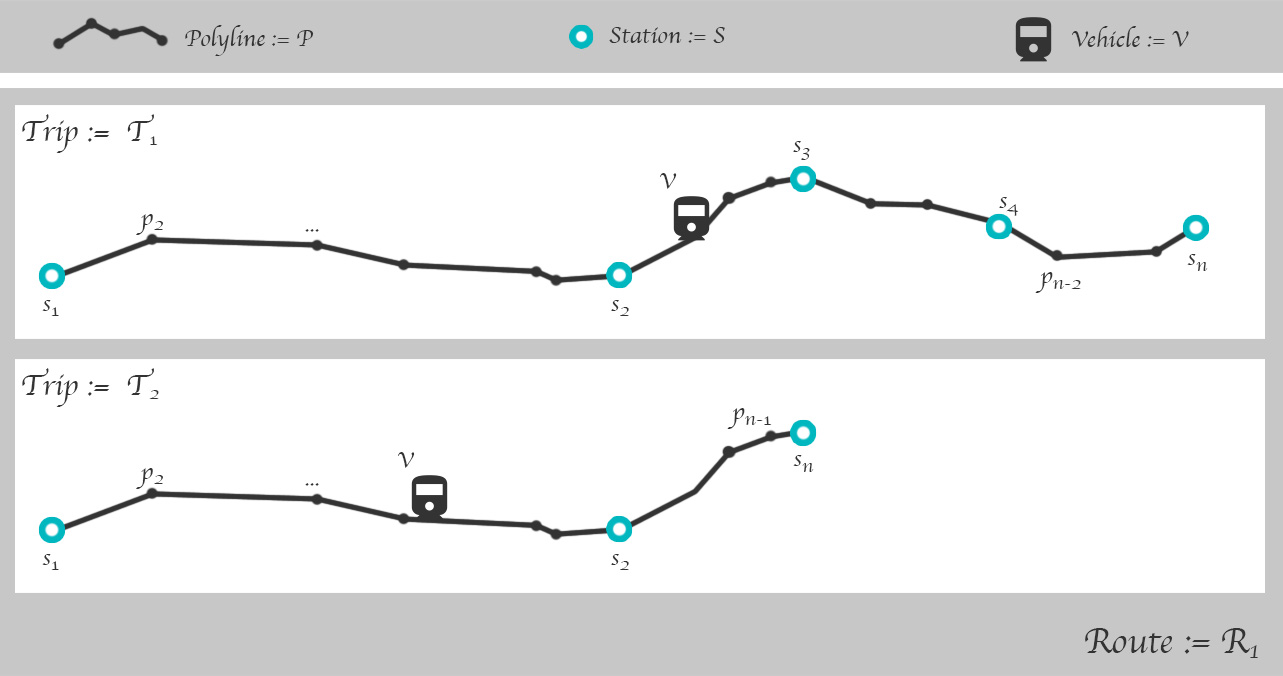
\includegraphics[width=\textwidth]{gtfs_viz.jpg}
          \caption{Grafische Veranschaulichung einer Route}
          \label{fig:gtfs_viz}
        \end{center}
      \end{figure}

      Abbildung \ref{fig:gtfs_viz} zeigt, dass eine Route zum Beispiel alle Trips einer U-Bahn-Linie erfasst. Eine U-Bahn-Linie muss dabei nicht immer an allen Stationen halten, sondern kann beispielsweise im Nachtbetrieb auch Stationen auslassen (zu sehen bei Trip $T_2$). Trotzdem werden nur diejenigen Trips in einer Route vereint, die dem selben Routenverlauf folgen.
    % subsubsection route (end)

% subsection begriffe (end)
    
  % section define (end)
\end{newpage}